% 244.jpg
\clearpage
\begin{exercises}

\exercise 三个质量分别为$ 100 $克、$ 200 $克和$ 300 $克的物
体,分别放在
\begin{wrapfigure}[9]{r}{12em}
  \centering
  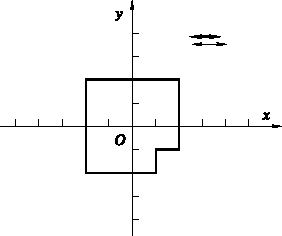
\includegraphics{figure/fig08.10}
  \caption{}
  \label{fig:08.10}
\end{wrapfigure}
$ \left(0, 30 \text {厘米} \right) $、
$ \left(40 \text{厘米}, 0 \right) $和
$ \left(0, 0 \right) $处,试求质心位置
$ \left( x _ { c } , y _ { c } \right) $。

\exercise 一均匀材料做成正方形,每边长$ 4.0 $米,在其一角上
切去一个边长为$ 1.0 $米的小正方形后,放置如图\ref{fig:08.10}形状,求余下
物体的质心位置$ \left( x _ { c } , y _ { c } \right) $。

\exercise 在半径为$ 50 $厘米的均匀圆盘上,有一半径为$ 30 $
厘米的圆孔,孔的中心距圆盘中心为$ 10 $厘米。求圆盘剩下部分的
质心位置。

\begin{wrapfigure}[8]{r}{12em}
  \centering
  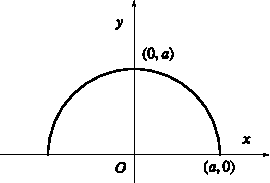
\includegraphics{figure/fig08.11}
  \caption{}
  \label{fig:08.11}
\end{wrapfigure}
\exercise 试求一个半径为$ a $的半圆形均匀平板的质心。它的安
放如图\ref{fig:08.11}所示。

\exercise 一质量为$ m $的人抓住一根挂在质量为$ M $的气球下
面的绳梯,最初气球和人相对于地面是静止的。试问:

(1)如果这人以相对于气球为$ v $的速率向上攀登,气球将向什么方
向运动?速率多大?

(2)这人停止攀登后,气球的运动状态如何?

\exercise 质量$ 70 $公斤的渔人站在船上,设船和渔人的总质量
为$ 200 $公斤,船静浮于水面。若渔人在船上向船头走$ 4.0 $米
后静止。试问:以岸为参考系,渔人走了多远(不计水的摩擦)?

\exercise 已知月球质量约为地球质量的$ 0.013 $倍,月、地中心
相距约为地球半径的$ 60 $倍,取地球半径为$ 6400 $公里。试问
月-地系统的质
% 245.jpg
心离地球中心多远?

\exercise \;$ m _ { 1 } = 12 $公斤和$ m _ { 2 } = 20 $公斤
的两个半径相同的、无相互作用的金属球,均静止地放在水平光滑的桌
面上,两球中心相距为$ l = 0.4 $米。今沿二球心联线方向在
$ m _ { 2 } $上加$ \vec { F } = 64 $公斤力,使
$ m _ { 2 } $远离$ m _ { 1 } $,试求:

(1)质心在未加力时的位置$ x _ { c } \left( 0 \right) $;

(2)在力$ \vec { F } $作用下质心的加速度;

(3)质心在加力后$ 3.0 $秒末移动的距离;

(4)以地球为参考系,在$ 3.0 $秒末体系的动能$ E _ { 0 } $;

(5)在质心参考系里,$ 3.0 $秒末体系的动能$ E ' $。

\exercise 有一质量为$ m _  { 1 } $、速度为$ v _ { 1 } $的
粒子,与一质量为$ m _  { 2 } $、原来静止的粒子发生完全非弹性
碰撞。试证明:这碰撞过程的机械能损失恰好等于在质心系中系统原来
的动能。

\exercise 有一质点系,起始时位置是$ m _ { 1 } = 4.0 $公斤,
坐标为$ \left( 1 , -3 \right) $;$ m _ { 2 } = 8.0 $公斤,
坐标为$ \left( 4 , 1 \right) $;$ m _ { 3 } = 4.0 $公斤,
坐标为$ \left( -2 , 2 \right) $,坐标单位为米。它们各个受力
是:$ \vec { F } _ { 1 } = 14 $牛顿,沿$ x $方向;
$ \vec { F } _ { 2 } = 16 $牛顿,沿$ y $方向;
$ \vec { F } _ { 3 } = 6 $牛顿,沿负$ x $方向。
它们分别在所受力的作用下独立运动。试求:

(1)各质点的加速度$ a _ { 1 } $,$ a _ { 2 } $,$ a _ { 3 } $;

(2)开始时的质心坐标;

(3)质心的加速度$ a _ { c } $。

\exercise 两球$ A $,$ B $质量相等
$ \left( m _ { A } = m _ { B } = m _ { c } \right) $,
在光滑的水平面上相碰,碰前速度分别为
$ v _ { A _ { 0 } } = 80 $米/秒,
$ v _ { B _ { 0 } } = 0 $;碰撞后分别沿与原$ A $球运动方向成
$ 30 ^ \circ $和$ 45 ^ { \circ } $角前进,如图\ref{fig:08.12}所示。试求:
\begin{figure}[h]
  \vspace{-0.5em}
  \centering
  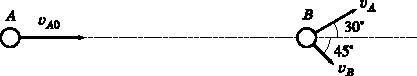
\includegraphics{figure/fig08.12}
  \vspace{-0.5em}
  \caption{}
  \label{fig:08.12}
\end{figure}
% 246.jpg

\clearpage
(1)碰撞后两球的速度$ v _ { A } $,$ v _ { B } $;

(2)因碰撞损失原有动能的百分之几?

\exercise 质量为$ m = 200 $克的弹性球撞到墙上,并被墙弹回。碰撞
前后速度的方向都和墙垂直,速度的大小都是$ v = 5.00 $米/秒。球
和墙的碰撞时间为$ \Delta t = 0.050 $秒。试求碰撞时间内球和墙的
相互作用力的平均值$ \overline { f } $。

\exercise 有一个$ 90 $公斤重的人,从$ 2.0 $米高处往地面跳,若他
每只脚踝骨的接触面积是$ 5.0 \text {厘米} ^ { 2 } $,已知人的骨头
抗压强度约为
$ 1.5 \times 10 ^ { 4 } \text {牛顿} / \text {厘米} ^ { 2 } $。
试问:

(1)若他与地面碰撞期间,他的质心向下移动$ 1.0 $厘米,那
么,他的踝骨会发生骨折吗?

(2)若他与地面碰撞期间,他的质心降低了$ 50 $厘米,他的踝骨
上单位面积平均接受多大冲力?

\exercise 质量为$ 3.0 $公斤的木块静止在水平桌面上,质量为
$ 5.0 $克的子弹沿水平方向射进木块。两者合在一起,在桌面上滑动
$ 25 $厘米后停止。木块与桌面的摩擦系数为$ 0.20 $。试求子弹原来
的速度。

\begin{wrapfigure}[6]{r}{7em}
  \vspace{-1.56em}
  \centering
  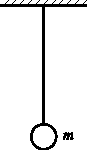
\includegraphics{figure/fig08.13}
  \caption{}
  \label{fig:08.13}
\end{wrapfigure}
\exercise 如图\ref{fig:08.13}所示,长为$ l = 30.0 $厘米,最
大强度为$ T = 1.00 $公斤力的绳子,系一质量为$ m = 500 $克的小
球,若$ m $原来静止不动。试问:要用多大的水平冲量作用在$ m $上,
才能把绳子打断?

\exercise 在放射性衰变中,一个$ \alpha $粒子(氦原子核)由最初
处于静止状态的$ ^{ 238 } \symrm{U} $的核中,以速率为
$ 1.4 \times 10 ^ { 7 }$米/秒被发射出来。试求剩余质量(
$ ^{ 234 } \symrm{Th} $)的反冲速率。

\exercise 如图\ref{fig:08.14}所示,小球$ m _ { 2 } $静止在光滑的半
圆形碗的底部,碗的半径为$ R $。另一小球$ m _  { 1 } $自碗边由静
止开始下落,并与$ m _ { 2 } $作
% 247.jpg
\begin{wrapfigure}[7]{r}{11.5em}
  %\vspace{-1.56em}
  \centering
  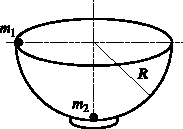
\includegraphics{figure/fig08.14}
  \caption{}
  \label{fig:08.14}
\end{wrapfigure}
完全非弹性碰撞。求:

(1)碰后的一瞬间,$ m _ { 1 } $和$ m _ { 2 } $对碗底的压力;

(2)\;$ m _ { 1 } $和$ m _ { 2 } $上升的最大高度。

\exercise 光滑平面上有两物体$ A $和$ B $,质量分别为
$ m _ { A } $和$ m _ { B } $。在一轻弹簧的作用下彼此
分开,各自以$ v _ { A } $和$ v _ { B } $
的速度作惯性运动。试证明分开之后,两物体的动能之比为
$ \dfrac { E _ { k A } } { E _ { k B } } = \dfrac { m _ { B } } { m _ { A } } $(图\ref{fig:08.15})。
\begin{figure}[h]
  \centering
  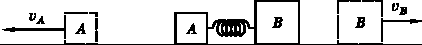
\includegraphics{figure/fig08.15}
  \caption{}
  \label{fig:08.15}
\end{figure}

\exercise 质量分别为$ m _ { 1 } = 5.0 $千克和
$ m _ { 2 } = 3.00 $千克的两球,分别以
速率$ v _ { 1 } = 12 $厘米/秒和$ v _ { 2 } = 4.0 $厘米/秒作对
头碰撞。求在下列两种情况下,碰撞后的速度:

(1)完全弹性碰撞

(2)完全非弹性碰撞。

\exercise 如图\ref{fig:08.16}所示,一个$ 60 $公斤的人站在$ 50 $公斤的平板车
\begin{wrapfigure}[8]{r}{15em}
  %\vspace{-1.56em}
  \centering
  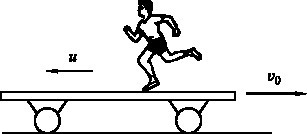
\includegraphics{figure/fig08.16}
  \caption{}
  \label{fig:08.16}
\end{wrapfigure}
上。最初车子以$ v _ { 0 } = 10 $米/秒的速度在水平光滑的轨道上
向右匀速运动。若此人对平板车以$ u=5.0 $米/秒的速度向左跑去。试问:

(1)车速将如何变化

(2)当他在左端跳下车后,车速又如何变化?

\exercise 如上题,但车上有两个人,各重$ 60 $公斤,车和人最初都静
% 248.jpg
止。试问:

(1)若一人相对车子以$ 5.0 $米/秒的速率首先跑到车的左端并跳下之后,
另一人相继再重复第一人的动作,最后车子的速度是多少?

(2)若两人同时相对车子以5.0米/秒的速率跑到车的左端并跳下,车子的速
度又是多少?

\exercise \;$ n $个体重均为$ m $的人,站在重为$ W $的平板车上。车
沿着平直路轨无摩擦地向前运动,速度为$ v _ { 0 } $。如果每个人都以
相对于车的速率$ u $向车后跑并跳下车,求在下列两种情况下,人都跳下
车后,车的速度$ v $。

(1)一个一个地跳(一个人跳离后,另一人才起步);

(2)全体同时跑,同时跳离车子。

\exercise 一个三级火箭,各级重量如下表所示,不考虑重力,火箭
的初速为零。
\begin{table}[h]
    \vspace{-0.8em}
    \zihao{-5}\fangsong
  \begin{tblr}{rightsep=1em,colspec={c*{3}{|X[r]}}}
    \toprule
    级\hspace{1em}别 & \SetCell{c}发射总质量    & \SetCell{c}燃\hspace{1em}料  & \SetCell{c}燃料外壳 \\
    \midrule
    一\hspace{1em}级 & $ 60 $吨\qquad & $ 40 $吨\qquad & $ 10 $吨\qquad  \\
    二\hspace{1em}级 & $ 10 $吨\qquad & $ 20/3 $吨\qquad & $ 7/3 $吨\qquad \\
    三\hspace{1em}级 & $ 1 $吨\qquad & $ 2/3 $吨\qquad & \\
    \bottomrule
  \end{tblr}
\vspace{-0.8em}
\end{table}

(1)若燃料相对于火箭喷出速率为$ u = 2500 $米/秒,每级燃料
外壳在燃料用完时将脱离火箭主体,设外壳脱离主体时,相对于主
体,其速度为零,只有当下一级火箭发动后,才将上一级的外壳
甩在后边。求第三级火箭的最终速率。

(2)若把$ 48 $吨燃料放在$ 12 $吨的外壳里组成一级火箭,问火箭
最终速率是多少?

\exercise 一宇宙飞船以恒速$ \vec { v } $在空间飞行,飞行过程中
遇到一股微尘粒子流,这些微尘粒子流以
$ \dfrac { \dif m } { \dif t } $的速率沉积在飞船上,尘粒
在
% 249.jpg
落到飞船之前的速度为$ \vec { u }$。在时刻$ t $,飞船的总质量
为$ M ( t ) $。试问:要保持飞船匀速飞行,需要多大的力?

\exercise 一雨滴的初始质量为$ M _ { 0 } $,在重力作用下、从静止
开始降落。假定此雨滴从云中得到质量,其质量的增长率正比于它的瞬时质
量和瞬时速率的乘积,即$ \dfrac { \dif M } { \dif t } = k M v $,
其中$ k $为常数。若忽略空气阻力,试证明雨滴的速率最终成为恒量,并
给出最终速率的表达式。

\begin{wrapfigure}[8]{r}{14.8em}
  %\vspace{-1.56em}
  \centering
  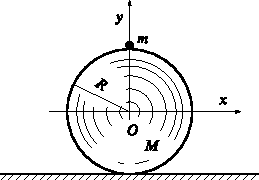
\includegraphics{figure/fig08.17}
  \caption{}
  \label{fig:08.17}
\end{wrapfigure}
\exercise 如图\ref{fig:08.17}所示,一半径为$ R $的光滑球,质量为$ M $,静
止在光滑的水平桌面上。在球顶点上有一质量为$ m $的质点。$ m $自
$ M $球自由下滑。试求$ m $离开$ M $之前的轨迹。

\exercise 一个水平运动的皮带将砂子从一处运到另一处,砂子经一垂直
的静止漏斗落到皮带

\begin{wrapfigure}[11]{r}{14.8em}
  \vspace{-1em}
  \centering
  \subfigure[\null]{
    \label{fig:08.18a}
    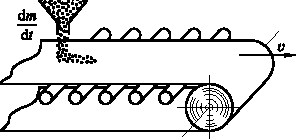
\includegraphics{figure/fig08.18a}
  } \\
  \subfigure[\null]{
    \label{fig:08.18b}
    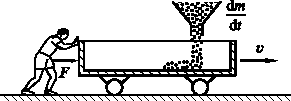
\includegraphics{figure/fig08.18b}
  }
  \caption{}
  \label{fig:08.18}
\end{wrapfigure}
\noindent 上,皮带以恒定的速率$ v $水平地运动着\lhbrak 见图\ref{fig:08.18a}
\rhbrak 。忽略机件各部位的摩擦。若砂子落到皮带上的速率是$ \dif m / \dif t $,试问:

(1)要保持皮带以恒定速率$ v $运动,水平总推力$ F $多大?
需要多大的功率?

(2)通过皮带提供的能量中有多少转化成砂子的动能?其余能量到哪里去了?

% 250.jpg
\clearpage
(3)若整个装置是:漏斗中的砂子落进以匀速$ v $在平直光滑轨
道上运动的货车里,\hspace{-0.2em}以上诸问的答案有改变吗\lhbrak \hspace{-0.2em}见图\ref{fig:08.18b}\hspace{-0.2em}\rhbrak ?

\exercise 线密度为$ \rho $、长度为$ l $的链条,用手提着一头,另
一头刚
\begin{wrapfigure}[11]{r}{11em}
  %\vspace{-1.56em}
  \centering
  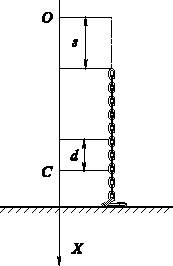
\includegraphics{figure/fig08.19}
  \caption{}
  \label{fig:08.19}
\end{wrapfigure}
好触及地面,静止不动。如图\ref{fig:08.19}所示。突然放手,使链条
自由下落。求证:当链条的上端下落的距离为$ s $时,链条作用在地面上
的力为$ 3 \rho g s $。

\lhbrak 提示:有两种求证方法:

(1)平台不仅要支持已落到台上并静止的链的重力($ s \rho g $),还要
使该时刻到达的链子动量降为零;

(2)求出链子质心的位置$ x _ { c } $:在图819中,设$ C $为链子
的质心位置,$ d $为质心到尚未落下链子($ l - s $)中心$ K $距离。
在质心系则质心坐标为零,故得,
$ 0 = \left( l - s \right) d - \left( \dfrac { l - s } { 2 } -d \right) s $,
由此求得
$ d = \dfrac { s \left( l - s \right) } { 2 l } $。
从几何关系知
$ x _ { c } = s + \dfrac { l - s } { 2 } + d = s + \dfrac { l } { 2 } - \dfrac { s ^ { 2 } } { 2 l } $,
对$ x _ { c } $求导即得
$ \ddot { x } _ { c } = \dfrac { 1 } { l }\left( \ddot { s } ^ 2 + s \ddot { s } \right)$,
再由$ m g - F = m \ddot { x } _ { c }$ 即得证\rhbrak 。

\exercise 两个物体的恢复系数$ r $定义为它们分开的速度和接触时
速度之比,$ 0 \leqslant r \leqslant 1 $。用它可解决一些既非
完全弹性又非完全非单性的碰撞问题。试证明:

(1)如果一个球和一个重的水平板之间的恢复系数为$ r $,则这球掉
下来经过$ n $次弹跳后,它反弹的高度为$ h _ { 0 } r ^ { 2 n } $,
其中$ h _ { 0 } $是此球开始掉下来的高度;
% 251.jpg

\clearpage
(2)两个质量分别为$ m _ { 1 } $和$ m _  { 2 } $的物体,
以恢复系数$ r $发生正面碰撞,则因碰撞失去的动能为质心系中动能的
$ \left( 1 - r ^ { 2 } \right) $倍。

\begin{wrapfigure}[9]{r}{13em}
  %\vspace{-1.56em}
  \centering
  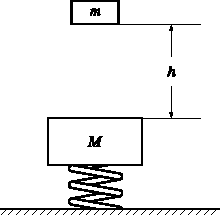
\includegraphics{figure/fig08.20}
  \caption{}
  \label{fig:08.20}
\end{wrapfigure}
\exercise 如图\ref{fig:08.20}所示,物体$ M $和弹簧原来都处于静止状态,弹
簧的倔强系数为$ k $。若有一质量为$ m $的物体从$ h $高度自由下落,
撞在物体$ M $上,设$ m $与$ M $作完全非弹性碰撞,求弹簧对地面的最
大压力$ N $(弹簧本身质量可忽略不计)。

\exercise 在光滑的水平桌面上,有$ A $和$ B $两个大滑块,它们的表
面都十分光滑,质量都是$ M $,高度都是$ h _ { 0 } $。$ A $滑块是
一段规则的三棱柱,$ B $滑块是凹面棱柱,$ B $凹面的下端与接触的桌
面相切(图\ref{fig:08.21})。在$ A $与$ B $的顶端各放置一个质量为$ m $的质点。
开始时,两个系统都静止,然后让$ m $自由下滑。设若$ m $滑至桌面时
没有跳动,都继续沿水平面滑行,试问:

(1)当质点$ m $与滑块分离后,两种情况的$ m $与$ M $的速度
$ v _ { A } $,$ V _ { A } $,$ v _ { B } $,$ V _ { B } $
各为多少?

(2)在这两种情况下,$ m $与$ M $分开后机械能的变化各为多少?
部分损失的机械能到哪里去了?
% TODO: \usepackage{graphicx} required
\begin{figure}[h]
  \centering
  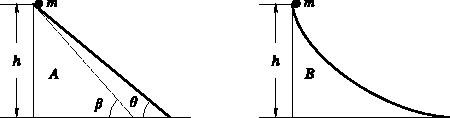
\includegraphics{figure/fig08.21}
  \caption{}
  \label{fig:08.21}
\end{figure}

\lhbrak 提示:对于$ A $的情况,$ m $实际上是沿图\ref{fig:08.21}中虚线到达
水
% 252.jpg
\clearpage\noindent
平面,$ m $的速度方向与水平面夹角为$ \beta $。$ m $与桌子平面的碰
撞在竖直方向是完全非弹性碰撞,系统只在水平方向保持动量守恒:
$ m v _ \text {斜} \cos \beta = M V _ { A }$。\rhbrak

\exercise 有一固定的光滑斜面,倾角为$ \theta $有一小物体,质量
为$ m $,从高$ H $处自由下滑,滑到斜面底$ C $点之后,继续沿水平
面平稳
\begin{wrapfigure}[7]{r}{14em}
  \vspace{1.5em}
  \centering
  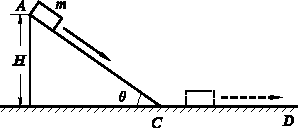
\includegraphics{figure/fig08.22}
  \caption{}
  \label{fig:08.22}
\end{wrapfigure}
地滑行(图\ref{fig:08.22})。设$ m $所滑过的路程全是光滑无摩擦的,试
求:

(1)\;$ m $到达$ C $点瞬间的速度$ v _ { c 0 } $;

(2)\;$ m $离开$ C $点的速度$ v _ { c } $;

(3)\;$ m $在$ C $点的动量损失及机械能量损失。

\exercise 一个小物体$ m $从高为$ h $、倾角为$ \theta $的斜面上
由静止开始下滑,然后又在水平面上继续前进一段距离$ s $后停止
(图\ref{fig:08.23})。设物体与斜面和平面的摩擦系数都为$ \mu _ { 0 } $。求:

\begin{wrapfigure}[7]{r}{14em}
  \vspace{1.5em}
  \centering
  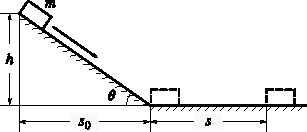
\includegraphics{figure/fig08.23}
  \caption{}
  \label{fig:08.23}
\end{wrapfigure}
(1)它在平面上前进的距离$ s $;

(2)当倾角$ \theta $很小(但$ \theta $角一定要大于摩擦角
$ \varphi $,即$ m g \sin \theta > \mu m g \cos \theta $,
$ \theta > \tg ^ { -1 } \mu = \varphi $)时,取
$ \cos \theta \approx 1 $,$\sin \theta \approx 0 $,将这结
果与第六章习题11的结果进行比较。

\exercise 一条质量为$ M $,长为$ l $的链子在桌子边缘上盘在一起。
链子的一端有极小的一段被推出桌子边缘,在重力作用下开始下落,
并把越来越多的链子从桌面拉出来。假定链子各部分在未被拉入
运动前速度一直保持为零,只是突然一下子以下落部分的速度开
% 253.jpg
始运动。试问:

(1)链子下落段长为$ x $时的速度是多少?

(2)当链子全部长度刚离开桌面的瞬间,原来的势能有多大
部分转化为链子的动能?

\exercise 一喷气式飞机的质量为$ M $,它的发动机把空气吸进来又
由机尾喷出去。喷出的气流对于飞机的速度是不变的,等于$ u $;每
秒钟喷出去的气的质量也是不变的,等于$ m $。设各处的摩擦力都
可略去,若在$ t = 0 $时飞机由静止出发并保持水平飞行,试求:

(1)飞机的速度$ v $与时间的关系;

(2)飞机的瞬时效率$ \eta $与$ u $和$ v $的关系,何时最大?最大
值$ \eta _ { \text { max } } $等于多少?

\end{exercises}